\authoredSection{markus}{Architektur}
	Nachdem zunächst in diesem Bericht bereits Konzepte und Ergebnisse erläutert wurden, gehen wir an dieser Stelle nun auf die Implementierung und technische Umsetzung der App ein. Im Fokus dabei steht die Architektur, die maßgeblich zum Ablauf der Entwicklung und zur Organisation der Kernkomponenten beiträgt.
	
	Unsere App soll den Kontakt zwischen einer Filialbank und seinen Kunden stärken. Da es sich bei KiBa lediglich um eine fiktive Bank handelt und die App auch anderen interessierten Banken vorgestellt werden soll, bietet es sich an, einen „Click-Dummy“ zu entwickeln. Dieser soll sich bereits wie eine vollwertige Banking-App bedienen lassen, die jedoch an keine reale Bank, respektive deren Datenbank, angeschlossen ist. Aufgrund dieser Rahmenbedingungen haben wir uns für die Architektur entschieden, die im Folgenden vorgestellt wird.

\subsection{Umsetzung des MVC-Ansatzes}
	Die Architektur muss uns dabei auf die Entwicklung der Kernfeatures fokussieren. Wenn nicht klar ist, wo welche Teile der Logik, der GUI oder anderer Komponenten zu platzieren sind, verzögert dies den Entwicklungsprozess und macht das Entwicklungsteam weniger produktiv.
	
	Daher fiel unsere Entscheidung auf den MVC-Ansatz; das heißt, wir versuchten unseren Code in Datenmodellierung, Visualisierung und Kontextualisierung zu gliedern.
	
	Auf oberster Ebene befinden sich deswegen nun die Ordner „Entities“ für die Modellierungsentitäten, „Services“ für Dienstleisterklassen, „Views“ für View-Controller und die die View repräsentierenden \texttt{xib}-Dateien und zuletzt ein „Library“-Ordner, der für alle Bereiche unterstützende Helferklassen sammelt.
	
	Innerhalb dieser Ordner haben wir darüber hinaus eine funktionale Substruktur erschaffen, die nach unseren Feature-Komponenten aufgebaut ist. Das hatte auch den positiven Nebeneffekt, dass kollaboratives Arbeiten am Projekt erleichtert wurde. Denn auf diese Weise war es nicht zwangsläufig für jede Einheit erforderlich, eine eigene Git-Branch zu eröffnen, da in den Ordnern gearbeitet werden konnte.

\subsection{Datenmodell}	
	Zur Modellbildung der App fiel unsere Entscheidung auf ein klassisches Entitäten-Be\-zieh\-ungs\-sys\-tem. Unser Weg zur Abstraktion einer Bank führt daher	über Klassen, die Modelle zu Objekten der realen Welt darstellen. Wie wir dabei vorgegangen sind, ist im Entitäten-Relationen-Diagramm unseres Datenmodells in Abbildung \ref{fig:ERDiagram} zu sehen.
	
	\begin{figure}[h]
	\centering
	\scalebox{.57}{
	\begin{tikzpicture}[node distance=1.5cm, every edge/.style={link}]
		% User
		\node[entity] (User) {User};
		\node[attribute] (User1) [above=of User] {userId} edge (User);
		\node[attribute] (User2) [above right=of User] {forename} edge (User);
		\node[attribute] (User3) [above left=of User] {surname} edge (User);
		\node[attribute] (User4) [right=of User] {password} edge (User);
		\node[isa] (isa) [below=1cm of User] {is a} edge[->] (User);
		
		% Consultant
		\node[entity] (Consultant) [below left=1cm and 2cm of isa] {Consultant} edge[->] (isa);
		\node[attribute] (Consultant1) [left=1cm of Consultant] {phoneNumber} edge (Consultant);
		\node[attribute] (Consultant2) [above=1cm of Consultant] {image} edge (Consultant);
		\node[attribute] (Consultant3) [above left=1cm of Consultant] {businessPosition} edge (Consultant);
		
		% Customer
		\node[entity] (Customer) [below right=1cm and 2cm of isa] {Customer} edge[->] (isa);
		\node[attribute] (Customer1) [above=of Customer] {authenticated} edge (Customer);
		
		% Address
		\node[relationship] (livesAt) [below left=of Customer] {lives at} edge node[cty] {1} (Customer);
		\node[entity] (Address) [below left=of livesAt] {Address} edge node[cty] {1} (livesAt);
		\node[attribute] (Address1) [left=of Address] {street} edge (Address);
		\node[attribute] (Address2) [right=of Address] {houseNr} edge (Address);
		\node[attribute] (Address3) [below=of Address] {postalCode} edge (Address);
		\node[attribute] (Address4) [above=of Address] {city} edge (Address);
		\node[attribute] (Address5) [above left=of Address] {coordinates} edge (Address);
		
		% Branch
		\node[relationship] (Located) [below left=1cm and 1.5cm of Address] {location} edge node[cty] {1} (Address);
		\node[entity] (Branch) [below left=.5cm and 0.75cm of Located] {Branch} edge node[cty] {1} (Located);
		\node[attribute] (Branch1) [below=of Branch] {name} edge (Branch);
		\node[attribute] (Branch2) [above left=of Branch] {bic} edge (Branch);
		\node[attribute] (Branch3) [below left=of Branch] {openHours} edge (Branch);
		\node[attribute] (Branch4) [left=of Branch] {phoneNumber} edge (Branch);
		\node[relationship] (leads) [above=4cm of Branch] {leads} edge node[cty, swap] {1} (Branch) edge node[cty] {n} (Consultant);
		
		% Account
		\node[relationship] (owns) [below=2cm of Customer] {owns} edge node[cty] {n} (Customer);
		\node[entity] (Account) [below=2cm of owns] {Account} edge node[cty] {1} (owns);
		\node[attribute] (Acc1) [above left=.3cm and 1cm of Account] {balance} edge (Account);
		\node[attribute] (Acc2) [above right=-.2cm and 1cm of Account] {accountNr} edge (Account);
		\node[attribute] (Acc3) [below right=-.5cm and 1cm of Account] {description} edge (Account);
		\node[attribute] (Acc4) [below left=-.5cm and 1cm of Account] {overDraft} edge (Account);
		
		% Transaction
		\node[relationship] (recipient) [below left=1cm and .5cm of Account] {recipient} edge node[cty, swap] {n} (Account);
		\node[relationship] (sender) [below right=1cm and .5cm of Account] {sender} edge node[cty] {n} (Account);
		\node[entity] (Transaction) [below right=1cm and .5cm of recipient] {Transaction} edge node[cty, swap] {1} (recipient) edge node[cty] {1} (sender);
		\node[attribute] (Transaction1) [below=of Transaction] {amount} edge (Transaction);
		\node[attribute] (Transaction2) [right=of Transaction] {date} edge (Transaction);
		
		% OpenHour
		\node[relationship] (opens) [below right=.2cm and 1.5cm of Branch] {opens} edge node[cty] {n} (Branch);
		\node[entity] (OpenHour) [below right=.2cm and 1.5cm of opens] {OpenHour} edge node[cty] {1} (opens);
		\node[attribute] (OpenHour1) [below left=of OpenHour] {openingTime} edge (OpenHour);
		\node[attribute] (OpenHour2) [below=of OpenHour] {closingTime} edge (OpenHour);
		\node[attribute] (OpenHour3) [below right=of OpenHour] {weekDay} edge (OpenHour);
		
		% Message
		\node[relationship] (inbox) [below right=.5cm and .5cm of Customer] {inbox} edge node[cty] {n} (Customer);
		\node[entity] (Message) [below right=.5cm and .5cm of inbox] {Message} edge node[cty] {1} (inbox);
		\node[attribute] (Message1) [below right=of Message] {description} edge (Message);
		\node[attribute] (Message2) [below left=.8cm of Message] {content} edge (Message);
		\node[attribute] (Message3) [above right=of Message] {sender} edge (Message);
		\node[attribute] (Message4) [above=of Message] {date} edge (Message);
		\node[attribute] (Message5) [right=of Message] {msgId} edge (Message);
	\end{tikzpicture}
}
	\caption{Entitäten-Relationen-Diagramm \label{fig:ERDiagram}}
\end{figure}
	
	Da gibt es zum einen die mit der Bank agierenden Benutzer, nämlich den Berater und den Kunden, die von einer gemeinsamen Klasse a\texttt{User} erben. Kunden, sprich \texttt{Customer}, besitzen mehrere Konten (\texttt{Account}) und erhalten mehrere Nachrichten (\texttt{Message}). Des weiteren verfügen sie, ebenso wie die Filialen,  über eine Adresse. Diese Filialen (\texttt{Branch}) wiederum werden von Beratern geleitet und sind zu verschiedenen Öffnungszeiten (\texttt{OpenHour}) besuchbar. Darüber hinaus finden Transaktionen (\texttt{Transaction}) zwischen Konten statt.

\subsection{Sicherheitsaspekte}
% MARKUS: kannst du die sicherheitsaspekte noch etwas weiter ausformulieren und sagen, wieso wir die daten nicht speichern, dass es egal ist, ob man gerade keinen zugriff hat und das banking später machen kann
%
	Ein wichtiger Aspekt, insbesondere im Hinblick auf den Umgang mit sensiblen Finanzdaten, ist die Sicherheit der App. Dabei ist es auch eine Aufgabe der Architektur, diese gewährleisten zu können. Im Folgenden erläutern wir die Schlüsse, die wir dementsprechend für die realistische Umsetzung zogen.
	
	Eine Fragestellung von essentieller Bedeutung für uns ist, was mit der App im Falle eines Diebstahls passieren würde. Da wir sowohl der Bank als auch dem Kunden gewährleisten müssen, dass ihre Daten sicher sind, haben wir das Risiko zu groß eingestuft, die Daten auf dem Gerät zu speichern. Das ist der Grund, weswegen alle Informationen nur im Zwischenspeicher des iPads liegen. Das hat für uns den Vorteil, dass beim Beenden der App alle Informationen verloren gehen, wenn der Kunde nicht mehr eingeloggt ist.
	
	Dass dies für den Kunden nachteilig wirkt, da er die Daten nicht umgehend zur Verfügung hat, ist unser meiner nach ein vernachlässigbarer Faktor. Wie oben bereits geschildert, stellen wir uns die Benutzung der App eher in ruhigen Bereichen vor, in denen in den meisten Fällen eine Internetverbindung existiert. Für den Self-Service gehen wir davon aus, dass die Bank ihren Kunden in der Filiale eine Internetverbindung zur Verfügung stellt. Sowieso sollte es eher im Interesse des Kunden sein, wichtige Finanzinformationen nur an Orten abzurufen, wo sie nicht vielen Menschen einsehbar sind.
	
	Zudem würde in einer über einen Dummy hinausgehenden Implementierung ein Time-Out-Token (ähnlich einem Cookie im Web-Umfeld) implementiert, welche nach beispielsweise zehn Minuten ohne Interaktion die Anwendung beendete. Außerdem gewährleistet der Authentifizierungsmechanismus, dass kritische Features serverseitig deaktiviert werden, indem der entsprechende Benutzer wieder auf nicht authentifiziert geschaltet wird. Dieser Mechanismus kann einerseits bei einer Verlustmeldung greifen, aber auch bei in irgendeiner Weise verdächtigem Verhalten, also ungewöhnlich viele oder große Transaktionen in bestimmten Zeiträumen.
	
	Wichtig ist außerdem, dass alle Daten direkt übertragen werden. Wir stellen uns ein direktes Protokoll wie eine \acs{REST}-Schnittstelle oder ein \acs{SOAP}-Verfahren zum Austausch der Informationen zwischen App und Server der Bank vor.
	
	Insbesondere letzter Punkt kann es erforderlich machen, dass die Datenquelle anpassbar sein muss. Eine Möglichkeit, das zu realisieren, erläutern wir im nächsten Abschnitt.

\subsection{Dependency Injection}
% MARKUS: beim dependency injection wäre es glaub ich noch gut, ein beispiel für die benutzung zu nennen. und den bootstrap code bitte noch etwas erklären a lá es werden variablen für alle typen erstellt, die je nach modus eine bestimmte instanz zugewiesen bekommen, die anschließend im dependency injector registriert werden
%
% MARKUS:und vllt initial das ziel davon nochmal genau nennen, dass man an beliebiger stelle im code auf diese registrierte abhängigkeit zugreifen kann, ohne verzweigen über den code zu verteilen
%
	Eine zentrale Anforderung der App-Architektur für uns ist außerdem das Austauschen von einzelnen Kernkomponenten, wie etwa die Datenschicht. Denn hierdurch kann aus dem Click-Dummy eine vollwertige Banking-App erschaffen werden können, ohne große Änderungen am Code vornehmen zu müssen. Sie muss uns den Eindruck nehmen, an eine echte Bank gebunden zu sein.
	
\begin{figure}[h]
	\centering
	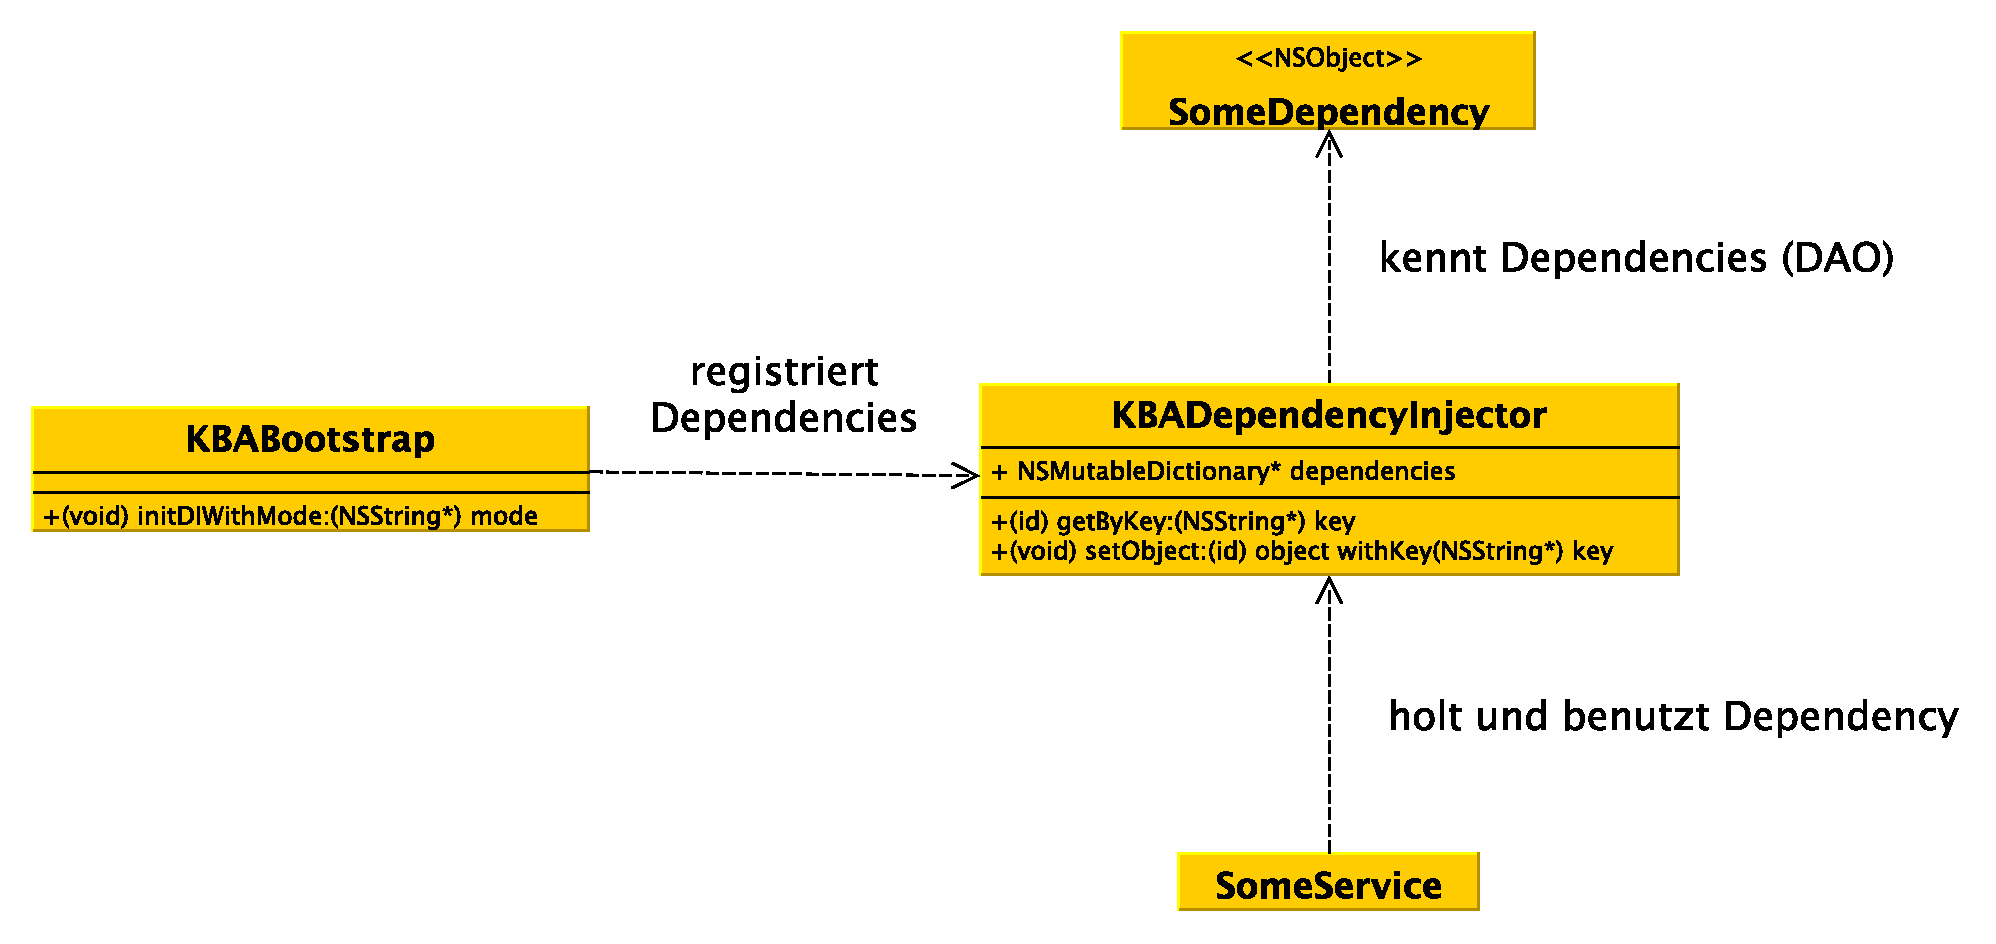
\includegraphics[scale=.25]{Pictures/uml-di}
	\caption{Klassendiagramm unserer Dependency Injection\label{fig:UmlDi}}
\end{figure}
	
	Daher ist für uns Dependency Injection als Entwicklungsmuster die Lösung dieses Problems. Wir haben es in einer reduzierten Form selbst implementiert. Dabei wird an einer zentralen Stelle im Quelltext, nämlich im \emph{Bootstrapping}, in den \lstinline{KBADependencyInjector} wie in Abbildung \ref{fig:UmlDi} sichtbar registriert, welche konkrete Implementierung einer Abhängigkeit in der Anwendung verwendet werden soll. Beim \lstinline{KBADependencyInjector} handelt es sich dabei nur um einen einfachen Schlüssel-Wert-Speicher.
	
	Der Bootstrapping-Prozess unserer App ist im Programmausdruck \ref{lst:Bootstrapping} wiedergegeben. Er zeigt an, wie zunächst lokale Variablen zu den generalisierten Protokollen typisiert sind, dann allerdings in einer bedingten Verzweigung entweder mit einer Dummy- oder einer konkreten Implementierung instantiiert werden. Abschließend werden die instantiierten Abhängigkeiten in den \lstinline{KBADependencyInjector} geschrieben. Beispielsweise wird für das Filial-\ac{DAO} eine lokale Variable des Typs \lstinline{id<KBABranchDao>} eingeführt, die im Entwicklungsmodus mit der Dummy-Implementierung \lstinline{KBABranchDaoDummy} und produktiv mit dem \lstinline{KBABranchDaoRest} instantiiert wird. Danach wird sie registriert.
	\pagebreak
	\lstinputlisting[label={lst:Bootstrapping}, caption={Der Bootstrapping-Vorgang}]{Listings/Bootstrapping}
	
\noindent	Wie zu erkennen ist, besitzt jedes \ac{DAO} ein Protocol, welches auf zwei Arten instanziiert werden kann. Dadurch erreichen wir, dass ein Programm auf verschiedene Art und Weise ausführbar ist. Die zentrale Registrierung der Abhängigkeiten hat außerdem den Vorzug, dass für eine andere Bank, die über eine andere Schnittstelle als (in diesem Fall) \ac{REST} verfügt, eine andere konkrete Implementierung nötig werden kann, die recht simpel nur an dieser Stelle im Code eingefügt werden muss. Man muss sich keine Gedanken mehr über weitere Abschnitte des Quelltext bei so einer Änderung machen.
	
	Ein weiterer Vorteil dieser Abstraktion ist die Testbarkeit der App. Dadurch, dass im Click-Dummy feste Daten hinterlegt sind, kann man sich zum Testen der App verschiedene Fälle erzeugen, die einfach in den jeweiligen \lstinline{*DaoDummy}s benutzt werden. Ein Beispiel für Unit Tests finden Sie im Programmausdruck \ref{lst:Unittest} in Kapitel \ref{sec:QMAusblick}.
	
	Darüber hinaus erlaubt uns dieses Verfahren auch die erleichterte Austauschbarkeit einzelner Komponenten. Wenn man dieses Verfahren auf andere Funktionen der App anwendet, insbesondere dann, wenn benutzerspezifische Elemente erforderlich sind, so ist es schnell möglich, eine White-Label-App zu erzeugen. Das heißt also wir können eine App schaffen, die auf verschiedene Kunden zugeschnitten werden kann. Dies hat für unseren Kunden T-Systems MMS in seiner Eigenschaft als Vermarkter den Vorteil, ihre App leicht auf Endkunden anpassen zu können.
	
	Wir haben festgestellt, dass die frühe Auseinandersetzung mit Fragen der Softwarearchitektur eine gute Entscheidung ist. Durch die Implementierung unserer eigenen Dependency-Injection und der zentralen Regelung von Abhängigkeiten an einem Ort haben wir eine dynamische und nachhaltige Methode geschaffen, unsere App sukzessive erweitern zu können.